%%%%%%%%%%%%%%%%%%%%%%%%%%%%%%%%%%%%%%%%%
% Beamer Presentation
% LaTeX Template
% Version 1.0 (10/11/12)
%
% This template has been downloaded from:
% http://www.LaTeXTemplates.com
%
% License:
% CC BY-NC-SA 3.0 (http://creativecommons.org/licenses/by-nc-sa/3.0/)
%
%%%%%%%%%%%%%%%%%%%%%%%%%%%%%%%%%%%%%%%%%

%----------------------------------------------------------------------------------------
%	PACKAGES AND THEMES
%----------------------------------------------------------------------------------------

\documentclass{beamer}

\mode<presentation> {

% The Beamer class comes with a number of default slide themes
% which change the colors and layouts of slides. Below this is a list
% of all the themes, uncomment each in turn to see what they look like.

%\usetheme{default}
%\usetheme{AnnArbor}
%\usetheme{Antibes}
%\usetheme{Bergen}
%\usetheme{Berkeley}
%\usetheme{Berlin}
%\usetheme{Boadilla}
%\usetheme{CambridgeUS}
%\usetheme{Copenhagen}
%\usetheme{Darmstadt}
%\usetheme{Dresden}
%\usetheme{Frankfurt}
%\usetheme{Goettingen}
%\usetheme{Hannover}
%\usetheme{Ilmenau}
%\usetheme{JuanLesPins}
%\usetheme{Luebeck}
\usetheme{Madrid}
%\usetheme{Malmoe}
%\usetheme{Marburg}
%\usetheme{Montpellier}
%\usetheme{PaloAlto}
%\usetheme{Pittsburgh}
%\usetheme{Rochester}
%\usetheme{Singapore}
%\usetheme{Szeged}
%\usetheme{Warsaw}

% As well as themes, the Beamer class has a number of color themes
% for any slide theme. Uncomment each of these in turn to see how it
% changes the colors of your current slide theme.

%\usecolortheme{albatross}
%\usecolortheme{beaver}
%\usecolortheme{beetle}
%\usecolortheme{crane}
%\usecolortheme{dolphin}
%\usecolortheme{dove}
%\usecolortheme{fly}
%\usecolortheme{lily}
%\usecolortheme{orchid}
%\usecolortheme{rose}
%\usecolortheme{seagull}
%\usecolortheme{seahorse}
%\usecolortheme{whale}
%\usecolortheme{wolverine}

%\setbeamertemplate{footline} % To remove the footer line in all slides uncomment this line
%\setbeamertemplate{footline}[page number] % To replace the footer line in all slides with a simple slide count uncomment this line

%\setbeamertemplate{navigation symbols}{} % To remove the navigation symbols from the bottom of all slides uncomment this line
}

\usepackage{graphicx} % Allows including images
\usepackage{booktabs} % Allows the use of \toprule, \midrule and \bottomrule in tables

\usepackage{graphicx} % Allows including images
\usepackage{booktabs} % Allows the use of \toprule, \midrule and \bottomrule in tables
\usepackage{framed}
%----------------------------------------------------------------------------------------
%	TITLE PAGE
%----------------------------------------------------------------------------------------

\title[Introduzione]{UML} % The short title appears at the bottom of every slide, the full title is only on the title page

\author{Claudio Menghi,  Srdan Krstic} % Your name
\institute[Deepse group] % Your institution as it will appear on the bottom of every slide, may be shorthand to save space
{
Politecnico di Milano \\ % Your institution for the title page
\medskip
\textit{menghi@elet.polimi.it,  srdan.krstic@polimi.it} % Your email address
}
\date{\today} % Date, can be changed to a custom date

\begin{document}

\begin{frame}
\titlepage % Print the title page as the first slide
\end{frame}

\begin{frame}
\frametitle{Overview} % Table of contents slide, comment this block out to remove it
\tableofcontents % Throughout your presentation, if you choose to use \section{} and \subsection{} commands, these will automatically be printed on this slide as an overview of your presentation
\end{frame}

%----------------------------------------------------------------------------------------
%	PRESENTATION SLIDES
%----------------------------------------------------------------------------------------


\begin{frame}
\frametitle{Esercizio 1: Veicolo}
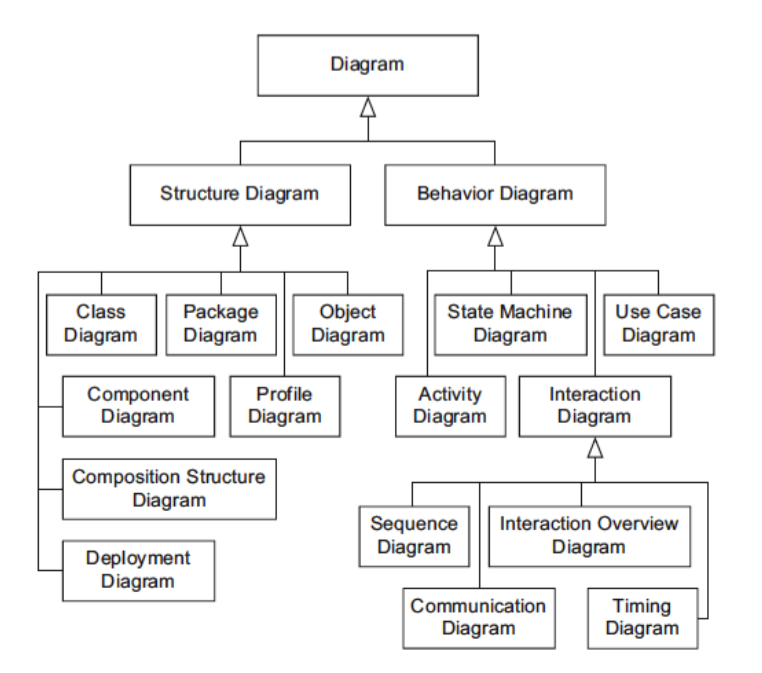
\includegraphics[scale=0.30]{Img/DiagrammiUML.png}

\end{frame}

\section{Esercizio 1: Veicolo}
\begin{frame}
\frametitle{Esercizio 1: Veicolo}
\begin{itemize}
\item Un Veicolo \`e composto da un Motore
\begin{itemize}
\item Veicolo: ha una targa e un numero di telaio
\item Motore: ha una cilindrata definita su n pistoni
\end{itemize}
\item  Un Pullman \`e un tipo di Veicolo che trasporta passeggeri
\begin{itemize}
\item Pullman: appartiene ad una societ\`a e dispone di n posti a sedere
\item Passeggero: \`e identificato da un nome e cognome
\end{itemize}
\end{itemize}
\end{frame}


\begin{frame}
\frametitle{Esercizio 1: UML Motore-Veicolo}
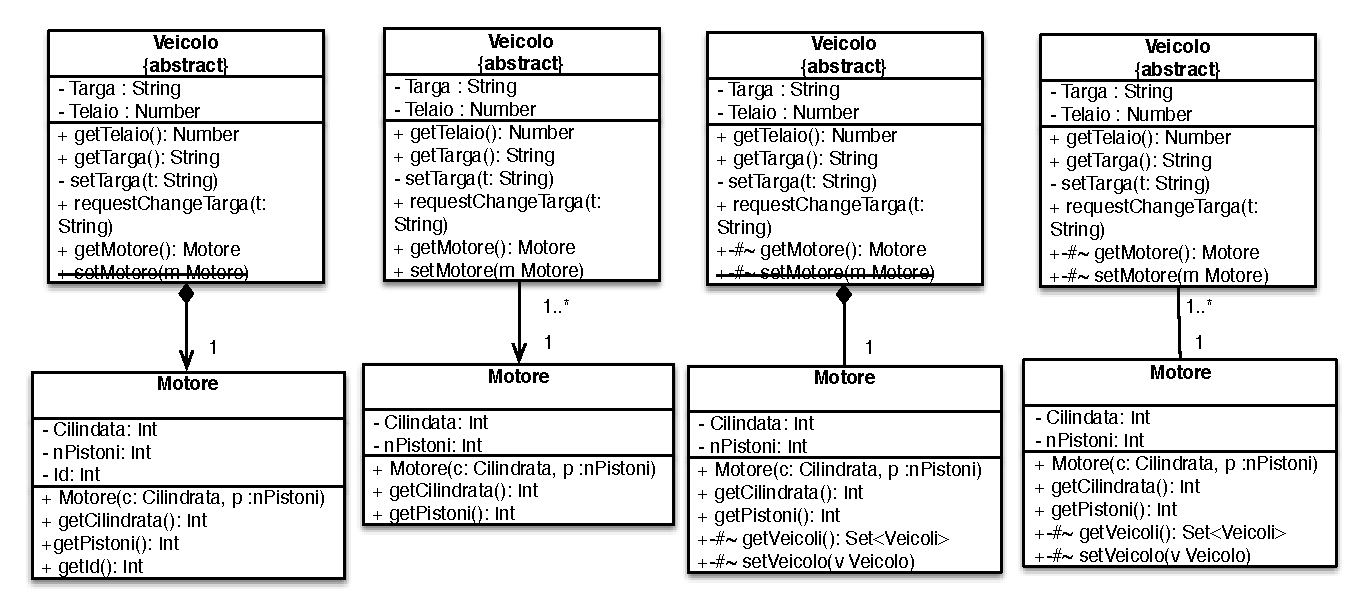
\includegraphics[scale=0.50]{Img/motoreveicolo.pdf}

\end{frame}

\begin{frame}
\frametitle{Esercizio 1: UML Pullman-Passeggero}
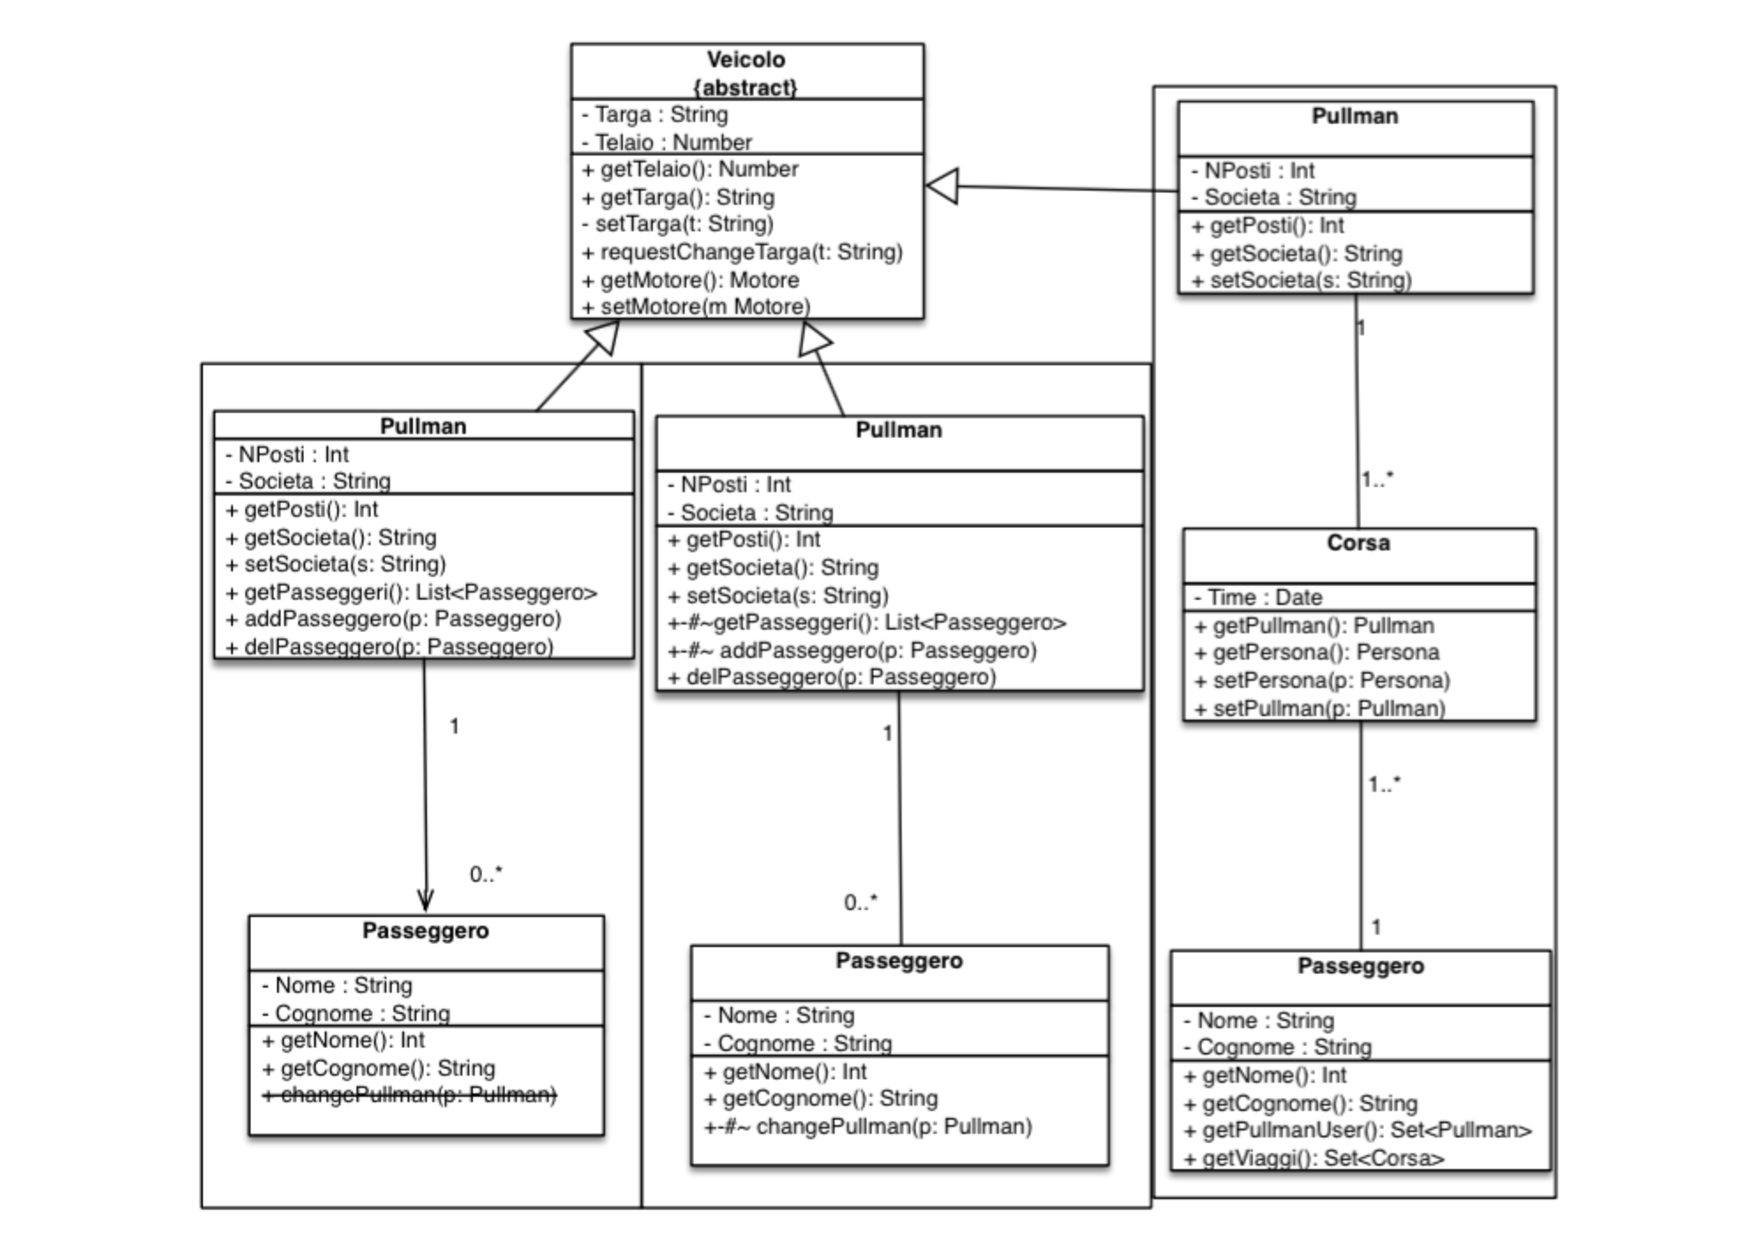
\includegraphics[scale=0.38]{Img/pullmanpasseggero.pdf}

\end{frame}


\section{Esercizio 2: Redazione}
\begin{frame}
\fontsize{9}{11}
\begin{itemize}
\item \emph{R1}: Nella redazione di una testata giornalistica ci sono tre tipi di giornalisti: gli editori, i reporter, ed i fotografi.
\item \emph{R2}: Ogni dipendente \`e caratterizzato da un nome e da un salario e ha diritto ad almeno un benefit (cio\`e un oggetto che viene concesso in uso al dipendente dall'azienda, ma che \`e di proprieta\`a dell'azienda).
\item \emph{R3}: Ci possono essere vari tipi di benefit: telefono cellulare, macchina fotografica, computer (che pu\`o essere o un portatile, o un palmare).
\item \emph{R4}: Tra i benefit ci possono anche essere degli apparecchi che hanno funzionalit\`a sia di telefono cellulare che di macchina fotografica.
\item \emph{R5}: Un telefono cellulare \`e caratterizzato da un numero di telefono, e offre la funzionalit\`a di chiamata di un altro numero, e di spedizione di un testo ad un altro telefono.
\item \emph{R6}: Se il telefono ha anche funzionalit\`a di macchina fotografica, permette anche di inviare immagini (sequenze di bit).
\item \emph{R7}: I fotografi hanno diritto, come benefit, ad esattamente una macchina fotografica.
\item \emph{R8}: Ci sono 2 tipi di reporter: i reporter junior e quelli senior.
\item \emph{R9}: I reporter junior hanno diritto ad esattamente un telefono cellulare; i reporter senior hanno invece diritto, ad un apparecchio con doppia funzionalita\`a celullare/macchina fotografica.
\item \emph{R10}: Un reporter pu\`o lavorare in coppia con un fotografo, e fa riferimento ad un editore.
\end{itemize}
\end{frame}

\begin{frame}
\frametitle{Esercizio 2: Redazione}
Dividiamo i requisiti in 3 categorie quelli che riguardano i benefit, quelli che riguardano i dipendenti e quelli che relazionano benefit e dipendenti
\begin{itemize}
\item requisiti che riguardano esclusivamente i benefit: \emph{R3}, \emph{R4}, \emph{R5}, \emph{R6}
\item requisiti che riguardano esclusivamente i dipendenti: \emph{R1}, \emph{R8}, \emph{R10}
\item requisiti che relazionano benefit e dipendenti: \emph{R2}, \emph{R7}, \emph{R9}
\end{itemize}
\end{frame}

\begin{frame}
\frametitle{Esercizio 2: Benefit}
\begin{itemize}
\item \emph{R3}: Ci possono essere vari tipi di benefit: telefono cellulare, macchina fotografica, computer (che pu\`o essere o un portatile, o un palmare).
\item \emph{R4}: Tra i benefit ci possono anche essere degli apparecchi che hanno funzionalit\`a sia di telefono cellulare che di macchina fotografica.
\item \emph{R5}: Un telefono cellulare \`e caratterizzato da un numero di telefono, e offre la funzionalit\`a di chiamata di un altro numero, e di spedizione di un testo ad un altro telefono.
\item \emph{R6}: Se il telefono ha anche funzionalit\`a di macchina fotografica, permette anche di inviare immagini (sequenze di bit).
\end{itemize}
\end{frame}

\begin{frame}
\frametitle{Esercizio 2: Benefit soluzione 1}
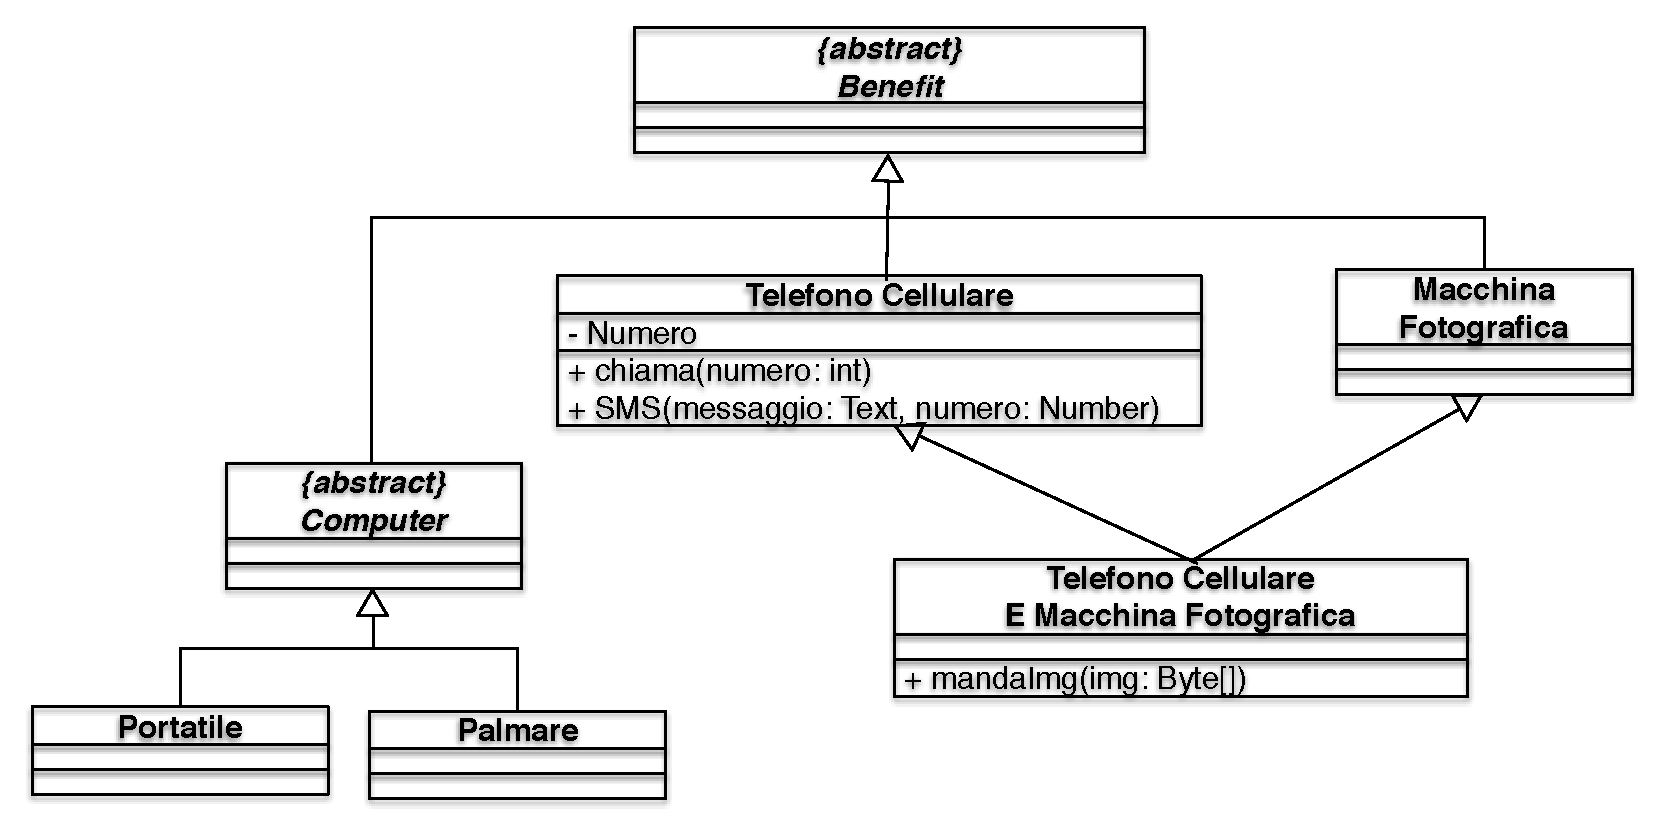
\includegraphics[scale=0.4]{Img/benefit1.pdf}
\end{frame}

\begin{frame}
\frametitle{Esercizio 2: Benefit soluzione 2a}
\includegraphics[scale=0.43]{Img/benefit2a.pdf}
\end{frame}

\begin{frame}
\frametitle{Esercizio 2: Benefit soluzione 2b}
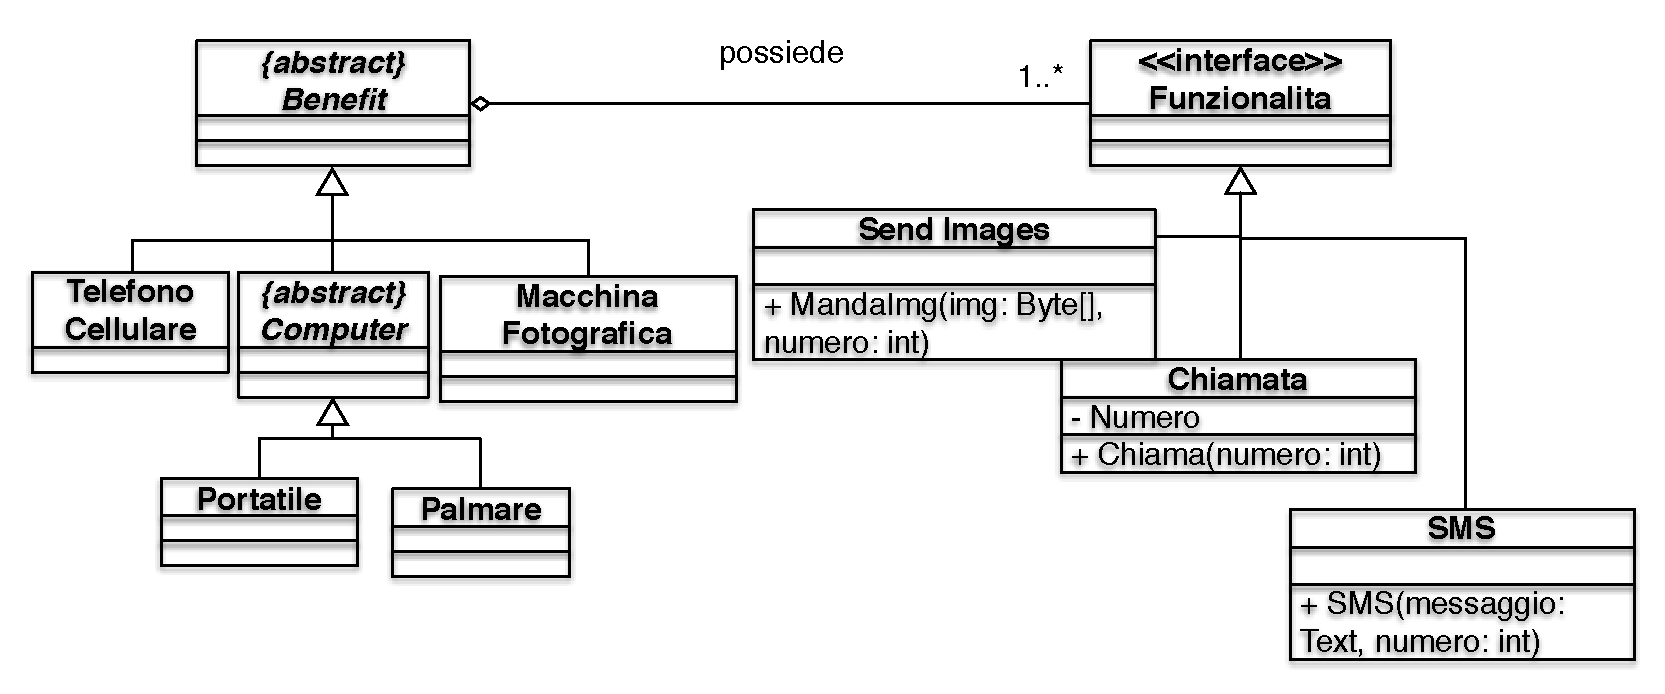
\includegraphics[scale=0.43]{Img/benefit2.pdf}
\end{frame}

%\begin{frame}
%\frametitle{Esercizio 2: Benefit soluzione 2c}
%\includegraphics[scale=0.43]{Img/benefit2c.pdf}
%\end{frame}
%\begin{frame}
%\frametitle{Esercizio 2: Benefit soluzione 3}
%\includegraphics[scale=0.43]{Img/benefit3.pdf}
%\end{frame}


\begin{frame}
\frametitle{Esercizio 2: Dipendente}
\begin{itemize}
\item \emph{R1}: Nella redazione di una testata giornalistica ci sono tre tipi di giornalisti: gli editori, i reporter, ed i fotografi.
\item \emph{R8}: Ci sono 2 tipi di reporter: i reporter junior e quelli senior.
\item \emph{R10}: Un reporter pu\`o lavorare in coppia con un fotografo, e fa riferimento ad un editore.
\end{itemize}
\end{frame}

\begin{frame}
\frametitle{Esercizio 2: Dipendente soluzione 1}
\includegraphics[scale=0.4]{Img/dipendente1.pdf}\\
\end{frame}

\begin{frame}
\frametitle{Esercizio 2: Dipendente soluzione 2}
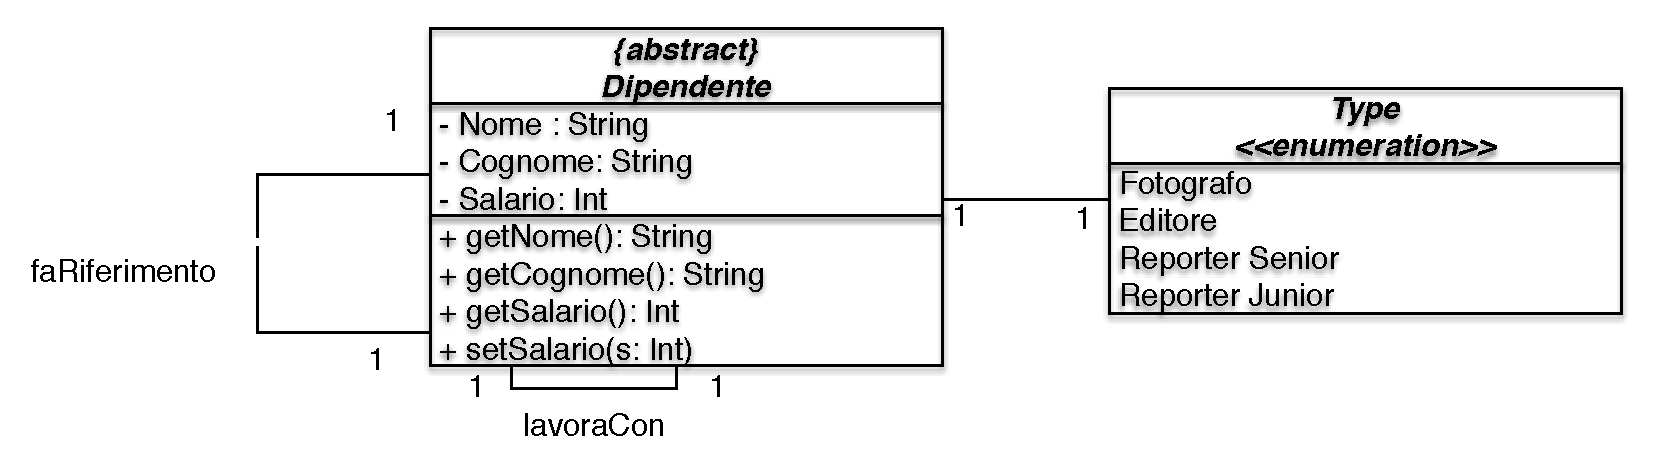
\includegraphics[scale=0.4]{Img/dipendente2.pdf}\\
\end{frame}


\begin{frame}
\frametitle{Esercizio 2: Dipendente-Benefit}
\begin{itemize}
\item \emph{R2}: Ogni dipendente \`e caratterizzato da un nome e da un salario e ha diritto ad almeno un benefit (cio\`e un oggetto che viene concesso in uso al dipendente dall'azienda, ma che \`e di proprieta\`a dell'azienda).
\item \emph{R7}: I fotografi hanno diritto, come benefit, ad esattamente una macchina fotografica.
\item \emph{R9}: I reporter junior hanno diritto ad esattamente un telefono cellulare; i reporter senior hanno invece diritto, ad un apparecchio con doppia funzionalita\`a celullare/macchina fotografica.
\end{itemize}
\end{frame}


\begin{frame}
\frametitle{Soluzione : Relazione Dipendenti-Benefit 1}
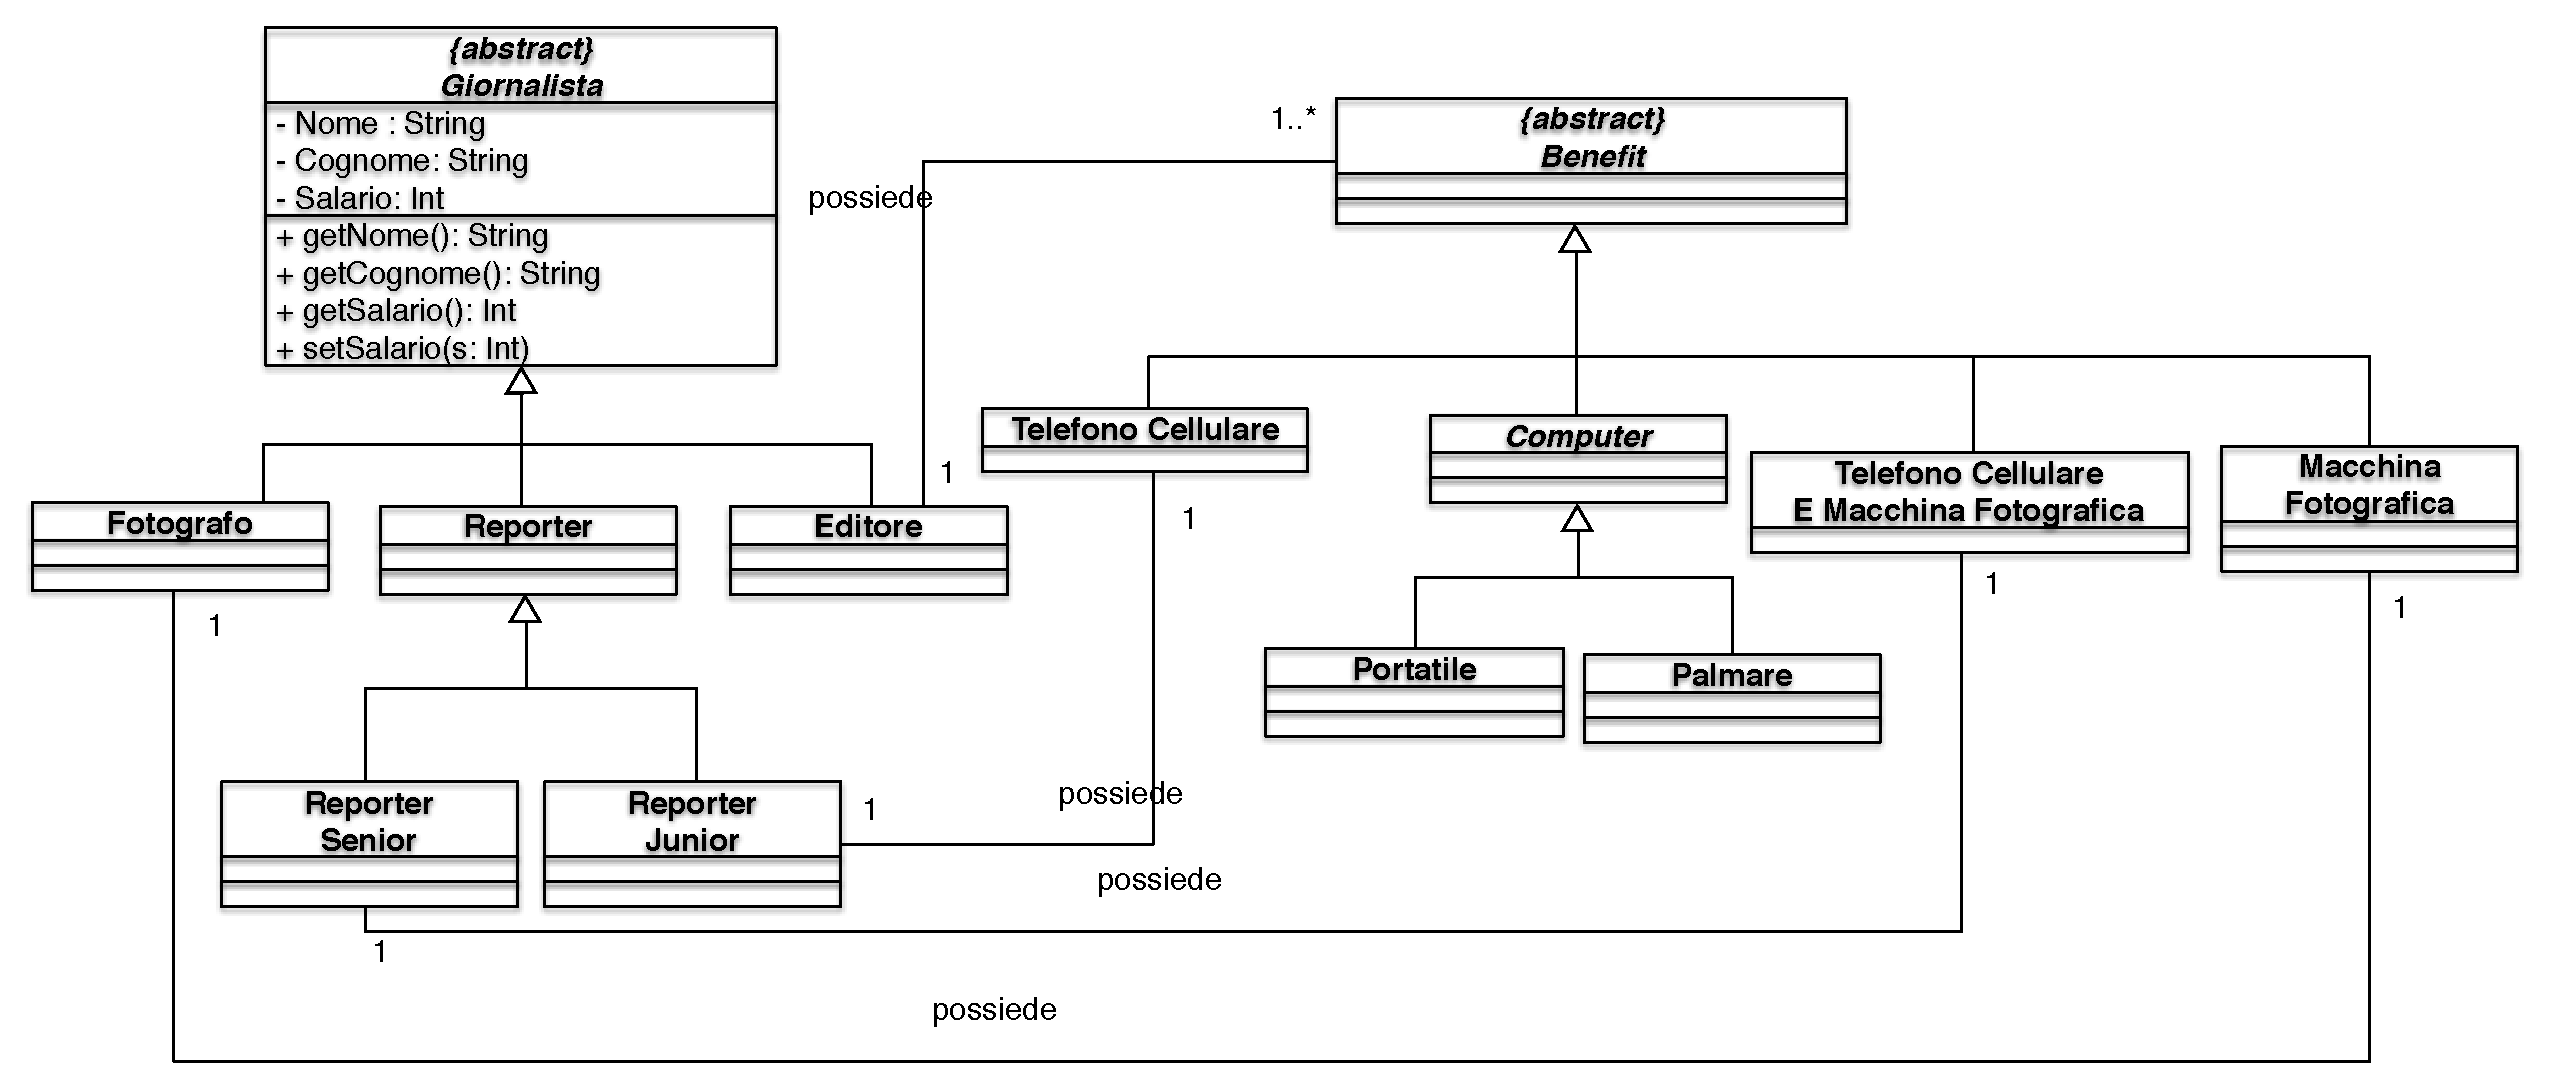
\includegraphics[scale=0.27]{Img/impiegatobenefit.pdf}
\end{frame}


%\begin{frame}
%\frametitle{Redazione sequence diagrams}
%Modellare con un sequence diagram le seguente sequenza di eventi:
%\begin{itemize}
%\item  Un reporter spedisce, mediante telefono cellulare, un testo al suo editor, il quale lo controlla e manda al reporter la conferma dell'accettazione dell'articolo.
%\item  L'editor, dopo aver confermato l'accettazione dell'articolo al reporter, manda l'articolo al servizio di composizione per l'inclusione nel giornale.
%\end{itemize}
%\end{frame}

\section{Esercizio 2: Rete Informatica}
\begin{frame}
\frametitle{Rete informatica}
Disegnare un diagramma delle classi UML che rappresenti una rete di computer.
\begin{itemize}
\item Questa si compone di nodi, i quali possono essere di due tipi: host e router.
\item Gli host sono connessi ad esattemente un router, mentre i router possono essere connessi ad un numero qualunque di host e ad almeno un altro router.
\item I nodi di una rete possono essere collegati tra loro mediante link fisici.
\item Un link fisico pu\`o collegare pi\`u host e pi\`u router tra loro.
\item Ogni connessione tra nodi della rete e link fisici è caratterizzata
da un indirizzo IP.
\item Un host nella rete pu\`o offrire dei servizi.
\item Ogni servizio, su un certo host, \`e caratterizzato da una porta.
\item Inoltre, ogni servizio si caratterizza per il tipo di protocollo su cui \`e trasportato, che pu\`o essere TCP o UDP.
\end{itemize} 
\end{frame}

\begin{frame}
\frametitle{Rete informatica}
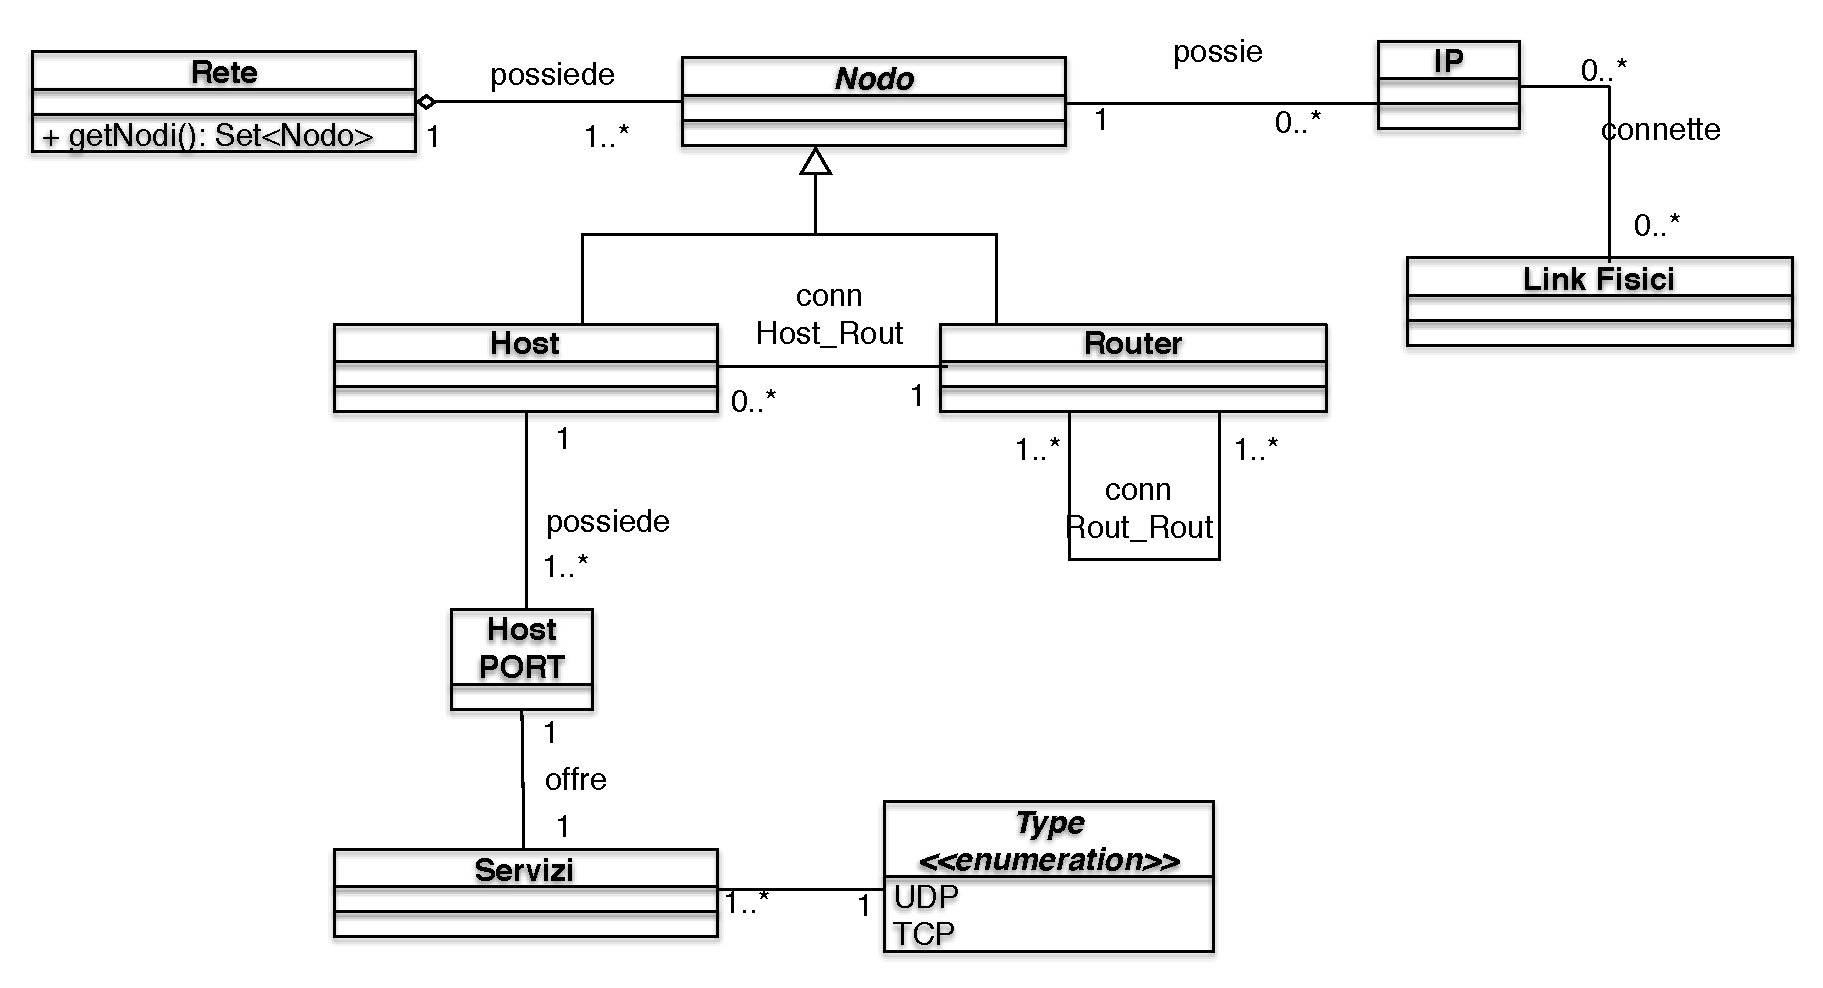
\includegraphics[scale=0.4]{Img/inf.pdf}
\end{frame}


\begin{frame}
\frametitle{Tools}
UML tools
\begin{framed}
\begin{itemize}
\item	\emph{architexa} e’ un plugin di eclipse che permette di generare una versione dei diagrammi UML partendo dal codice;
\item	\emph{Visual paradigm} ottimo per generare UML da codice e codice per UML, ma non e’ integrato con eclipse (nel caso MAC) ed e' a pagamento (ottimo tool)
\item  \emph{StarUML}, \emph{Modelio},  \emph{Papyrus},  \emph{UML2 Tools}
\item	ci sono tool non legati al codice, e.g., per mac e’ possibile scaricare degli stencil per omnigraffle, per windows c’e’ Visio
\item \textbf{www.draw.io}
\end{itemize}

Abbiamo un tool nella lista dei tool da valutare
\begin{itemize}
\item \emph{Magic Draw} (scaricabile dal sito del poli http://www.software.polimi.it/software-download/studenti/magic-draw/)
\end{itemize} 
\end{framed}
\end{frame}


\section{Introduction}
\begin{frame}
\frametitle{Design}
What is a good design?
\end{frame}

\begin{frame}
\frametitle{Design}
What is a good design?
\begin{framed}
A design the good if the cost of changing the design is minimal.
\end{framed}
\end{frame}


\begin{frame}
\frametitle{Design}
How to create a good design?
\end{frame}

\begin{frame}
\frametitle{Design}
How to create a good design?
\begin{framed}
Take your time.\\
Review the design.\\
Keep it simple.\\
\begin{itemize}
\item keep it focuses
\item solves only real problem we know about
\item is easy to understand
\end{itemize}
\end{framed}
\end{frame}

\begin{frame}
\frametitle{Design}
Complexity
\begin{framed}
\begin{itemize}
\item Inherent
\item Accidental
\end{itemize}
\end{framed}
\end{frame}

\subsection{Design Principles}

\begin{frame}
\frametitle{Design Principles}
Open Close Principle
\begin{framed}
Le entit\`a del software (le classi, i moduli e le funzioni) devono essere \emph{aperte all'estensione} e \emph{chiuse alle modifiche}\\
\end{framed}
\end{frame}

\begin{frame}
\frametitle{Design Principles}
\includegraphics[scale=0.5]{Img/ocpbad.pdf}
\end{frame}

\begin{frame}
\frametitle{Design Principles}
\includegraphics[scale=0.5]{Img/ocpgood.pdf}
\end{frame}


\begin{frame}
\frametitle{Design Principles}
Dependency Inversion Principle
\begin{framed}
I moduli di alto livello non devono dipendere direttamente dai moduli di basso livello. Entrambi devono dipendere da delle astrazioni.
\end{framed}
Quando delle classi di alto livello devono accedere a delle risorse di basso livello (disco I/O etc..) \`e conveniente
\end{frame}


\begin{frame}
\frametitle{Design Principles}
Single Responsibility Principle
\begin{framed}
A class should have only one reason to change.
\end{framed}
\end{frame}

\begin{frame}
\frametitle{Design Principles}
Liskov's Substitution Principle
\begin{framed}
Derived types must be completely substitutable for their base types.
\end{framed}
\end{frame}




%----------------------------------------------------------------------------------------

\end{document} 